\documentclass[prx, twocolumn, superscriptaddress, amsmath, amssymb, floatfix, longbibliography, nofootinbib, notitlepage]{revtex4-1}
\usepackage{amsmath}
\usepackage{amssymb}
\usepackage{color}
\usepackage[colorlinks]{hyperref}
\usepackage{tikz}
\usetikzlibrary{through,hobby}
\usetikzlibrary{patterns.meta}
\usetikzlibrary{calc}

\begin{document}

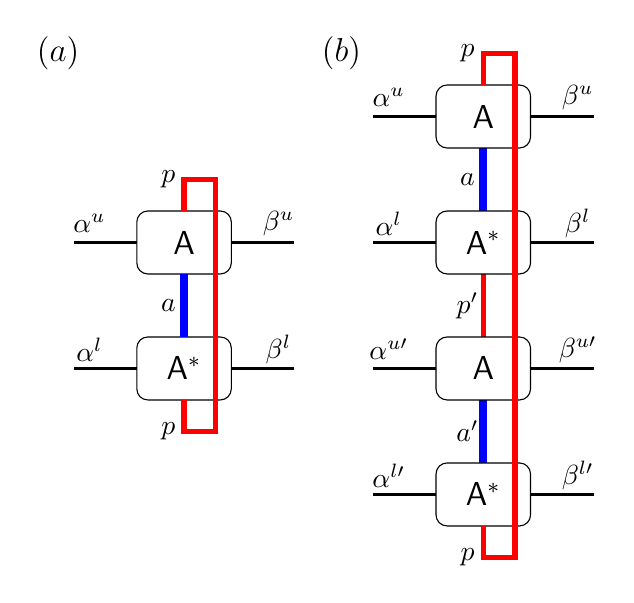
\begin{tikzpicture}[scale=0.8]
\tikzstyle{sergio}=[rectangle,draw=none]
\filldraw[fill=white, draw=black, rounded corners] (-0.25,-0.5)--(1.25,-0.5)--(1.25,0.5)--(-0.25,0.5)--cycle;
\filldraw[fill=white, draw=black, rounded corners] (-0.25,-2.5)--(1.25,-2.5)--(1.25,-1.5)--(-0.25,-1.5)--cycle;
\path (0.5,0) node [style=sergio]{\large $\mathsf{A}$};
\path (0.5,-2) node [style=sergio]{\large $\mathsf{A}^*$};
\draw[line width=2pt, color=red] (0.5,0.5) -- (0.5,1) -- (1,1) -- (1,-3) -- (0.5,-3) -- (0.5,-2.5);
\draw[line width=3pt, color=blue] (0.5,-1.5) -- (0.5,-0.5);
\path (0.25,1) node [style=sergio]{$p$};
\path (0.25,-1) node [style=sergio]{$a$};
\path (3,3) node [style=sergio]{\large $(b)$};
\path (-1.5,3) node [style=sergio]{\large $(a)$};
\path (0.25,-3) node [style=sergio]{$p$};
\draw[line width=1pt] (1.25,-2) -- (2.25,-2);
\draw[line width=1pt] (-0.25,-2) -- (-1.25,-2);
\draw[line width=1pt] (1.25,0) -- (2.25,0);
\draw[line width=1pt] (-0.25,0) -- (-1.25,0);
\draw[line width=2pt, color=red] (5.25,-0.5) -- (5.25,-1.5);
\draw[line width=3pt, color=blue] (5.25,1.5) -- (5.25,0.5);
\draw[line width=3pt, color=blue] (5.25,-2.5) -- (5.25,-3.5);
\draw[line width=1pt] (3.5,2) -- (7,2);
\draw[line width=1pt] (3.5,0) -- (7,0);
\draw[line width=1pt] (3.5,-2) -- (7,-2);
\draw[line width=1pt] (3.5,-4) -- (7,-4);
\path (-1,0.3) node [style=sergio]{$\alpha^u$};
\path (-1,-1.7) node [style=sergio]{$\alpha^l$};
\path (2,0.3) node [style=sergio]{$\beta^u$};
\path (2,-1.7) node [style=sergio]{$\beta^l$};
\path (3.75,-3.7) node [style=sergio]{$\alpha^{l\prime}$};
\path (3.75,-1.7) node [style=sergio]{$\alpha^{u\prime}$};
\path (3.75,0.3) node [style=sergio]{$\alpha^l$};
\path (3.75,2.3) node [style=sergio]{$\alpha^u$};
\path (6.75,-3.7) node [style=sergio]{$\beta^{l\prime}$};
\path (6.75,-1.7) node [style=sergio]{$\beta^{u\prime}$};
\path (6.75,0.3) node [style=sergio]{$\beta^l$};
\path (6.75,2.3) node [style=sergio]{$\beta^u$};
\filldraw[fill=white, draw=black, rounded corners] (4.5,1.5)--(6,1.5)--(6,2.5)--(4.5,2.5)--cycle;
\filldraw[fill=white, draw=black, rounded corners] (4.5,-0.5)--(6,-0.5)--(6,0.5)--(4.5,0.5)--cycle;
\path (5.25,2) node [style=sergio]{\large $\mathsf{A}$};
\path (5.25,0) node [style=sergio]{\large $\mathsf{A}^*$};
\filldraw[fill=white, draw=black, rounded corners] (4.5,-2.5)--(6,-2.5)--(6,-1.5)--(4.5,-1.5)--cycle;
\filldraw[fill=white, draw=black, rounded corners] (4.5,-4.5)--(6,-4.5)--(6,-3.5)--(4.5,-3.5)--cycle;
\path (5.25,-2) node [style=sergio]{\large $\mathsf{A}$};
\path (5.25,-4) node [style=sergio]{\large $\mathsf{A}^*$};
\draw[line width=2pt, color=red] (5.25,-4.5) -- (5.25,-5) -- (5.75,-5) -- (5.75,3) -- (5.25,3) -- (5.25,2.5);
\path (5,3) node [style=sergio]{$p$};
\path (5,-5) node [style=sergio]{$p$};
\path (5,-1) node [style=sergio]{$p'$};
\path (5,1) node [style=sergio]{$a$};
\path (5,-3) node [style=sergio]{$a'$};
\end{tikzpicture}

\end{document}